%%%%%%%%%%%%%%%%%%%%%%%%%%%%%%%%%%%%%%%%%%%%%%%%%%%%%%%%%%%%%%%%%
\newpage
\section[Determinanten]{Determinanten}
\Einleitung{Ein zentrales Thema in diesem Semester sind Determinanten, für die wir mit der Betrachtung von Gruppen ja schon die Vorarbeit geleistet hatten.\\ Letzte Woche hatten wir Endomorphismen als einen Spezialfall der linearen Abbildungen kennengelernt - diese bilden aus einem Vektorraum $V$ wieder nach $V$ ab!\\
Bei Anwendung des gaußschen Algorithmus auf die darstellende Matrix von Endomorphismen (diese ist quadratisch!) ergibt sich auf natürliche Weise ein Objekt, mit dem wir die Endomorphismen charakterisieren können: Die Determinante.\\
Bereits nächste Woche werden wir sehen, dass die Determinante bei der Bestimmung spezieller mit linearen Abbildungen verknüpfter Werte nützlich ist.\\
Zudem schauen wir uns an, wie man Matrizen invertieren kann und welche Feinheiten man dabei beachten muss.}
\subsection{Hinführung}
Wir versuchen, uns dem am Anfang sehr abstrakten Konzept der Determinante anhand von zwei Problemen zu nähern, sodass die Definition sinnvoll erscheint:\\
Betrachtet man Endomorphismen,\footnote{zunächst einmal auf einem endlichdimensionalen Vektorraum $V$, da wir sonst keine darstellenden Matrizen mehr finden können} so stellt sich schnell die Frage, wie man (wenn überhaupt) eine Umkehrabbildung finden kann. Diese Fragestellung können wir auf die Inversion der darstellenden Matrix zurückführen. Lasst uns dazu ein Beispiel betrachten:
\begin{Beispiel}
{Invertieren einer Matrix}
Wir betrachten eine lineare Abbildung $F:\mathbb{R}^2\to\mathbb{R}^2$, die durch
\begin{equation*}
    F\Matrix{x\\y}=A\Matrix{x\\y}=\Matrix{a&b\\c&d}\Matrix{x\\y}=\Matrix{x'\\y'}
\end{equation*}
definiert sei. Hierbei sei $A$ die darstellende ($2\times 2$)-Matrix bezüglich der kanonischen Basis.\\
Wir können uns stattdessen auch das folgende lineare Gleichungssystem angucken:
\begin{eqnarray*}
    I:&\quad&ax+by=x'\\
    II:&\quad&cx+dy=y'
\end{eqnarray*}
anschauen. Eine Inversion der Matrix entspricht dem Umstellen dieses Systems nach $x$ und $y$. Probiert euch selbst gern daran, ihr solltet schließlich bei
\begin{eqnarray*}
I:&\quad& x=\frac{1}{ad-bc}(dx'-by')\\
II:&\quad &y=\frac{1}{ad-bc}(-cx'+ay')
\end{eqnarray*}
herauskommen,\footnote{Unten haben wir dieses Ergebnis noch einmal als \textit{Cramersche Regel} festgehalten.} sodass wir in Matrixdarstellung die Form
\begin{equation*}
    \Matrix{x\\y}=\frac{1}{ad-bc}\Matrix{d&-b\\-c&a}\Matrix{x'\\y'}=:\frac{1}{\det A}\Matrix{d&-b\\-c&a}\Matrix{x'\\y'}
\end{equation*}
Diesen Vorfaktor identifizieren wir mit der Determinante, wir haben also
\begin{equation}
    \det A=\det\Matrix{a&b\\c&d}=ad-bc.
\end{equation}
Für diese $2\times2$-Matrix war das ja noch entspannt, aber auch beim Invertieren von anderen $n\times n$-Matrizen taucht sie auf.
\end{Beispiel}
\blue{Hier taucht die Determinante im Nenner auf. Dies ist ein erstes Zeichen, dass wir aufpassen müssen, wenn $\det A=0$ ist. In diesem Fall sind Matrizen nicht invertierbar und lineare Gleichungssysteme nicht mehr garantiert lösbar.}
\begin{Beispiel}{Anwendung des Gauß-Algorithmus}
Genauso taucht die Determinante auf, wenn wir den Gauß-Algorithmus auf die Matrix anwenden:
\begin{equation}
    \Matrix{a&b\\c&d}\overset{(II)\cdot a-c\cdot(I)}{\longrightarrow}\Matrix{a&b\\0&ad-bc}=\Matrix{a&b\\0&\det A}
\end{equation}
Diese Umformungen verwenden wir auch, wenn wir ein Gleichungssystem der Form $Ax=b$ lösen.\\
Dieses Prinzip können wir auf eine $n\times n$-Matrix erweitern und erhalten ganz analog als letzten Eintrag die Determinante:
\begin{center}
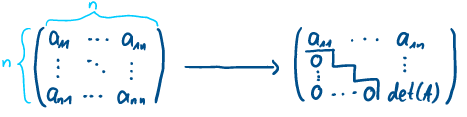
\includegraphics[width=.5\textwidth]{Dateien/00/14DeterminanteNKreuzN.PNG}
\end{center}
Leider wird es hierbei aber schnell sehr kompliziert, die Determinante zu berechnen.
\end{Beispiel}
\begin{Satz}{Rechenregel}{Cramersche Regel}
Wir halten fest:\\
Ein Gleichungssystem der Form $A\xvec=\bvec$, wobei\\ $A=\Matrix{a&b\\c&d}\in\Met(2,\mathbb{K})$ und $\bvec=\Matrix{e\\f}\in\mathbb{K}^2$, bzw.
\begin{equation*}
    ax+by=e,\quad cx+dy=f,
\end{equation*}
wird (falls $\det A=ad-bc\neq0$) gelöst durch
\begin{align*}
    x=\frac{1}{\det A}(ed-bf)\\
    y=\frac{1}{\det A}(af-ce).
\end{align*}
\end{Satz}
Ein weiteres Beispiel (das Volumen eines Parallelotops) findet ihr im Anhang dieses Kapitels, Abschnitt \ref{ssec:14AnhangParallelotop}.



\subsection{Kurze Wiederholung zu Gruppen und deren Anwendung}
Auch wenn ihr letztes Semester bereits die wichtigsten Begriffe für Gruppen kennengelernt habt, wollen wir, bevor es richtig losgeht, hier nochmal daran erinnern. Diese neue algebraische Struktur (neben Körpern und Vektorräumen) braucht ihr im Rahmen der Mathevorlesungen vor allem zur präzisen Formulierung der Determinanten. Aber auch in der Physik spielen sie eine tragende Rolle, zum Beispiel wenn es um die Beschreibung von Symmetrien (Drehung, Verschiebung, Spiegelung etc.) geht. Daher handelt es sich hier keineswegs um ein Nischenthema sondern um ein mathematisches Werkzeug, dass zu immensen Fortschritten im Verständnis der Natur geführt hat. \\

Also dann legen wir mal los: was war denn noch gleich eine Gruppe? Dazu schauen wir uns erstmal die trockene Definition an:
\begin{Wiederholung}
{Gruppen}
Eine Gruppe besteht aus einer Menge $G$ und einer Verknüpfung $\cdot:G\times G \mapsto G$, die folgende Eigenschaften erfüllen: \\

\begin{itemize}
    \item $(u\cdot v)\cdot w = u\cdot (v\cdot w) \qquad \forall u,v,w \in G$ \qquad (Assoziativität)
    \item $\exists e\in G: u\cdot e = e\cdot u = u \qquad \forall u\in G$ \qquad (Existenz des neutralen Elements)
    \item $\forall u\in G \, \exists u^{-1} \in G\,: u\cdot u^{-1} = u^{-1} \cdot u = e$ \qquad (Existenz des inversen Elements) \\
\end{itemize} 

Ist die Verknüpfung zusätzlich noch kommutativ, spricht man von einer \red{abelschen Gruppe}.
\end{Wiederholung}
Wie sehen jetzt aber Mengen aus, die diese Voraussetzungen erfüllen und was macht sie so besonders? Dazu schauen wir und mal ein paar Beispiele an, die ihr auch schon aus dem letzten Semester kennen solltet:
\begin{Beispiel}
{Besondere Gruppen}
\begin{enumerate}
    \item Bijektive Abbildungen bilden zusammen mit der Komposition \glqq $\circ$ \grqq eine Gruppe. Dass die Komposition Assoziativität erfüllt, haben wir in Mathe 1 gesehen. Mit der Identität $\Id$ und der Umkehrabbildung sind auch neutrales und inverses Element gegeben. Wir schreiben die Gruppe als:
    \begin{equation*}
        \Bij(X)=\Menge{\varphi : X \rightarrow X}{\varphi \text{ bijektiv}}.
    \end{equation*}
    Ist $X$ eine endliche Menge, nennt man $\sigma \in \Bij(X)$ eine \red{Permutation}.
    \item Die symmetrische Gruppe \red{(wichtig!)} ist definiert als
    \begin{equation*}
        S_{n} = \Bij(\{1,...,n\}).
    \end{equation*}
    Sie enthält Abbildungen, die alle n Elemente einer Gruppe nehmen und umordnen (permutieren).
    \item Ist $X=V$ ein Vektorraum, nennt man 
    \begin{equation*}
        \Aut(V) = \Bij(V)
    \end{equation*}
    die Automorphismengruppe.
    \item Ist $V$ endlichdimensional, dann ist 
    \begin{equation*}
        \GL(V) = \Aut (V)
    \end{equation*}
    die allgemeine lineare Gruppe (\underline{G}eneral \underline{L}inear Group).
    Ist $V=\mathbb{K}^{n}$, dann gilt:
    \begin{equation*}
        \GL(n,\mathbb{K}) = \Menge{A\in \Met (n,\mathbb{K})}{\ker (A)=0}
    \end{equation*}
    \item Zusätzlich (nicht in der Vorlesung!) betrachten wir noch die spezielle lineare Gruppe, die definiert ist durch
    \begin{equation*}
        \SL(n,\mathbb{K}) = \Menge{A\in \Met (n,\mathbb{K})}{\det (A)=1}.
    \end{equation*}
    Sie enthält alle orientierungs- und volumenerhaltenden Abbildungen und ist gelegentlich ganz nützlich.
    \item (Vorgriff) Aus physikalischer Sicht spielen auch die unitäre und spezielle unitäre Gruppe mit $\mathbb{K}=\mathbb{C}$ eine wichtige Rolle
    \begin{equation*}
        \text{U}(n)=\Menge{A\in\Met (n,\mathbb{C})}{AA^{\dagger}=A^{\dagger}A=\mathds{1}_{n}} 
    \end{equation*}
    \begin{equation*}
        \text{SU}(n)=\Menge{A\in \Met (n,\mathbb{C})}{AA^{\dagger}=A^{\dagger}A=\mathds{1}_{n} \land \det (A) = 1}
    \end{equation*}
    Tatsächlich bilden diese beiden Gruppen die Grundlage des Standardmodells der Teilchenphysik! Solltet ihr mit dem Symbol $\dagger$ (sprich \glqq{}dagger\grqq{}) noch nichts anfangen können, seid beruhigt: ihr lernt es gleich zu beginn dieser Vorlesung kennen. Es bedeutet, dass man die Matrix komplex konjugiert und transponiert.
\end{enumerate} 
\end{Beispiel}
Anhand dieser Beispiele seht ihr schon, dass die Gruppenstruktur in unter Anderem durch bijektive Abbildungen gegeben ist. Bijektivität ist deswegen wichtig, da wir ein inverses Element, sprich eine Umkehrabbildung brauchen. Geben wir ein paar weitere Schranken vor, enthalten wir speziellere Gruppen wie die symmetrische Gruppe oder die Automorphismengruppe. \\
Permutationen, die Elemente einer endlichen Menge umordnen, oder auch Symmetrietransformationen, sind am Ende nichts anderes als bijektive Abbildungen. Eine Umordnung kann man immer zurückordnen und eine Transformation, wie zum Beispiel eine Drehung oder eine Verschiebung, lässt sich immer zurücktransformieren. Hoffentlich macht das die Bedeutung von Gruppen etwas klarer. \\

Als nächstes wollen wir nochmal ein paar wichtige Begriffe, die im Zusammenhang mit Gruppen stehen, wiederholen.
\begin{Wiederholung}
{Gruppenhomomorphismus}
Ein Gruppenhomomorphismus $\varphi: G \rightarrow H$ zwischen zwei Gruppen $G$ und $H$ erfüllt die Bedingung
\begin{equation*}
    \varphi (a\cdot b)=\varphi (a) \cdot \varphi (b) \quad a,b \in G 
\end{equation*}
\end{Wiederholung}
\begin{Wiederholung}
{Transposition}
Eine \red{Transposition} ist eine bestimmte Permutation, die wie folgt definiert ist:
\begin{equation*}
    \tau_{ij} := \Matrix{1 & ... & i & ... & j & ... & n \\ 1 & ... & j & ... & i & ... & n}.
\end{equation*}
Sie vertauscht also die Elemente $i$ und $j$ einer gegebenen (nummerierten) Anzahl von Elementen miteinander.
\end{Wiederholung}
\begin{Wiederholung}
{Signum}
Das \red{Signum} einer Permutation $\sigma$ ist ein Gruppenhomomorphismus $\epsilon : S_{n} \rightarrow \{-1,1\}$, der definiert ist durch
\begin{equation*}
    \epsilon (\sigma) := \prod_{i<j} \frac{\sigma(j)-\sigma(i)}{j-i}
\end{equation*}
Jede Permutation lässt sich durch eine Verkettung von Transpositionen darstellen:
\begin{equation*}
    \sigma = \tau_{1}\circ\tau_{2} \circ ... \circ \tau_{k}.
\end{equation*}
Dabei ist die Anzahl $k$ der Transpositionen nicht eindeutig. Was aber sehr wohl eindeutig ist, ist ob $k$ gerade oder ungerade ist. Man kann tatsächlich zeigen, dass das Signum auch berechnet werden kann durch
\begin{equation*}
    \epsilon(\sigma)=(-1)^{k},
\end{equation*}
was deutlich leichter ist als die Formel, die wir davor hatten.
\end{Wiederholung}
\begin{Wiederholung}
{Zykel}
Ein \red{Zykel} ist eine weitere spezielle Permutation, die wie folgt definiert ist:
\begin{equation*}
    \zeta = \Matrix{1 & 2 & ... & n} = [2\,3\, ... \, n] = \Matrix{1 & 2 & ... & n-1 & n \\ 2 & 3 & ... & n & 1}.
\end{equation*}
Er bewirkt also eine zyklische Vertauschung aller Elemente. Möglicherweise ist euch der Begriff schonmal über den Weg gelaufen, falls ihr das Levi-Civita-Symbol (Epsilon-Tensor) im ersten Semester behandelt habt.
\end{Wiederholung}
Falls ihr zu diesen Begriffene weitere Beispiele sehen wollt, könnt ihr gerne in die Notizen zum Mathe 1 - Tutorium schauen. Hier wollen wir uns jetzt ein paar Anwendungen der Gruppentheorie anschauen. An ersterer Stelle steht dabei natürlich die Definition der Determinante (siehe Kap. \ref{ssec:Determinante}).


\subsection{Determinanten - Eindeutig, alternierend, linear}\label{ssec:Determinante}
Wir charakterisieren die Determinante zunächst folgendermaßen:
\begin{Def}
{Determinante}
Die \red{Determinante} einer $n\times n$-Matrix $\det:\Met(n,\mathbb{K})\to\mathbb{K}$ ist eine Abbildung, die die folgenden Eigenschaften hat:
\begin{enumerate}
    \item $\det$ ist linear\footnote{für alle Spaltenvektoren aus $\mathbb{K}^n$ und $\lambda\in\mathbb{K}$} in jeder Spalte:\blue{
    \begin{equation*}
        \det\Matrix{a_{11}\cdots\lambda a_{1i}+b_{1i}\cdots a_{1n}\\\vdots\quad \quad\vdots\\a_{n1}\cdots \lambda a_{ni}+b_{ni}\cdots a_{nn}}=\lambda\det\Matrix{a_{11}\cdots a_{1i}\cdots a_{1n}\\\vdots\quad\quad\vdots\\a_{n1}\cdots a_{ni}\cdots a_{nn}}+\det\Matrix{a_{11}\cdots b_{1i}\cdots a_{1n}\\\vdots\quad\quad\vdots\\a_{n1}\cdots b_{ni}\cdots a_{nn}}
    \end{equation*}}
    \item $\det$ ist alternierend:\\
    \blue{$\Rightarrow\det A=0$, falls zwei Spalten von $A$ gleich sind}
    \item Die Determinante der Einheitsmatrix ist $\det(\mathds{1}_n)=1$.
\end{enumerate}
Es stellt sich heraus, dass diese Abbildung \red{eindeutig} ist.\\
Spannenderweise existiert eine Funktion, die diese Axiome erfüllt und zudem eindeutig ist.\\
Sie ist durch die monströse \red{Leibnizsche Determinantenformel} gegeben. Sei dazu $A\in \Met (n, \mathbb{K})$:
\begin{equation*}
    \det (A) = \sum_{\sigma \in S_{n}} \epsilon (\sigma) a_{\sigma(1)1}\cdot ... \cdot a_{\sigma(n)n}.
\end{equation*}
Anhand dieser Formel wird klar, warum wir Gruppen für die Berechnung von Determinanten brauchen. Wir müssen hier nämlich über sämtliche Permutationen der symmetrischen Gruppe $S_{n}$ summieren! Leider sind das genau $n!$ Stück, womit man für größere Matrizen eine enorme Anzahl an Summanden bekommt (bei 6x6-Matrizen sind es zum Beispiel stolze 720!). Zum Glück habt ihr ja schon leichtere Methoden kennengelernt, mit denen man die Determinante schneller ausrechnen kann.
\end{Def}
\subsubsection{Wichtige Sätze zu Determinanten}
Wie wir wissen, können wir jedem Endomorphismus\footnote{Lineare Abbildung von $V\to V$} $F\in\End(V)$ bezüglich einer Basis\footnote{Linear unabhängige Familie von $n$ Vektoren, die $V$ aufspannen, d. h. dass jeder Vektor von $V$ eine eindeutige Darstellung als Linearkombination der Basisvektoren hat.} von $V$ eine \red{darstellende Matrix} $A$ zuordnen.
\begin{Satz}{Satz}
{Determinante eines Endomorphismus}
Die Determinante eines Endomorphismus $F\in\End(V)$ mit darstellender Matrix $A$ ist unabhängig von der Basis von $V$, d. h.
\begin{equation}
    \det F=\det A.
\end{equation}
\end{Satz}
\begin{Satz}
{Satz}{Satz zum Rang}
Ist der Rang einer Matrix $A\in\Met(n,\mathbb{K})$ $\rg A\neq n$, so ist $\det A=0$.
\end{Satz}
\blue{Zusammen mit dem vorhergehenden Satz sehen wir also:\\
Ein Endomorphismus ist genau dann ein Automorphismus, wenn die Determinante seiner darst. Matrix $\neq0$ ist.\\
Zudem liefert dies eine Aussage über die Invertierbarkeit von Matrizen: $A^{-1}$ existiert, wenn $\det A\neq 0$.}

\begin{Satz}
{Satz}{Determinantenmultiplikationssatz}
Für $A,B\in\Met(n,\mathbb{K})$ gilt:
\begin{equation}
    \boxed{\det(A\cdot B)=\det (A)\cdot\det(B)}.
\end{equation}
Somit folgt:\\
Die Determinante $\det:\GL(n,\mathbb{K})\to\mathbb{K}\setminus\{0\}$ ist ein Gruppenhomomorphismus.\footnote{Hierbei beschränken wir uns auf $\GL(n,\mathbb{K})$, d. h. Automorphismen zwischen endlichdimensionalen Vektorräumen, deren Determinante ungleich 0 wird. Wir müssen uns darauf beschränken, da $(\mathbb{K},\cdot)$ keine Gruppe ist, $(\mathbb{K}\setminus\{0\},\cdot)$ aber schon.}
\end{Satz}
\begin{Satz}
{Satz}{Inverse einer Determinante}
Für alle Gruppenhomomorphismen gilt $\phi(a^{-1})=\phi(a)^{-1}$. Somit gilt für alle\\
$A\in\GL(n,\mathbb{K})$:
\begin{equation}
    \det(A^{-1})=\det(A)^{-1}.
\end{equation}
Dies ist wohldefiniert, da $A\in\GL(n,\mathbb{K})$ per Definition bijektiv ist und somit eine Umkehrabbildung $A^{-1}$ besitzt und die Determinante nicht verschwindet.
\end{Satz}
\begin{Beispiel}
{Inverse einer Matrix}
Sei $A=\Matrix{2&2\\3&4}$. Die inverse Matrix ist\footnote{später lernt ihr das Werkzeug kennen, wie man diese bestimmt.} $A^{-1}=\Matrix{2&-1\\-\frac{3}{2}&1}$, denn $A^{-1}A=\mathds{1}_2=AA^{-1}$.\\
Es gilt:
\begin{align*}
    \det(A^{-1})&=2-(-1)(-3/2)=2-\frac{3}{2}=\frac{1}{2}\\
    \det(A)^{-1}&=(2\cdot 4-3\cdot 2)^{-1}=2^{-1}=\frac{1}{2}.
\end{align*}
\end{Beispiel}


\subsubsection{Berechnung von Determinanten}
Okay, wir haben dieses Objekte jetzt charakterisiert, aber wie gehen wir zur Berechnung vor?\\
Die folgende Formel ist eher unhandlich:
\begin{Satz}
{Berechnungsvorschrift}{Explizite Formel für die Determinante}
Für $A=(a_{ij})_{i=1...n,\,j=1...n}\in\Met(n,\mathbb{K})$ ist die Summe die folgende Summe:
\begin{equation}
    \det A=\sum_{\sigma\in S_n}\epsilon(\sigma)a_{\sigma(1)1}\cdots a_{\sigma(n)n}
\end{equation}
Jetzt sehen wir also, wofür wir das ganze Gruppengedöns gebraucht haben.\footnote{Es hat natürlich noch viele weitere Anwendungen, Gruppentheorie ist ein spannender Zweig der Mathematik.}
\end{Satz}
Wir hatten gesehen, dass $S_n$ genau $n!$ Elemente hat - die Summe setzt sich also wahnsinnig schnell aus sehr vielen Termen zusammen. Daher sind vereinfachende Regeln praktisch.\\
Lasst uns aber zunächst mit dieser Schreibweise vertraut machen:
\begin{Beispiel}
{Reproduktion der 2x2-Formel (1/2)}
$S_2$ enthält nur die Permutationen $\sigma_1=[12]$ und $\sigma_2=[21]$. Es ist $\epsilon(\sigma_1)=(-1)^2=1$ und $\epsilon(\sigma_2)=(-1)^1=-1$, da $\sigma_2$ sich aus genau einer Transposition darstellen lässt.\\
Also ist die Determinante von $A\in\Met(2,\mathbb{K})$ einfach nur
\begin{equation}
    \det A=\sum_{i=1}^{2}\epsilon(\sigma_i)a_{\sigma_i1}a_{\sigma_i2}=\epsilon(\sigma_1)a_{11}a_{22}+\epsilon(\sigma_2)a_{21}a_{12}=a_{11}a_{22}-a_{21}a_{12}.
\end{equation}
Dies ist die bekannte Formel, die wir auch schon in den Einführungsbeispielen schon gesehen hatten.
\begin{equation}
\end{equation}
\end{Beispiel}
\begin{Beispiel}
{Reproduktion der 1 für die Einheitsmatrix (2/2)}
Für die Einheitsmatrix $(e_{ij})_{i=1...n,\,j=1...n}=E=\mathds{1}_n\in\Met(n,\mathbb{K})$ erfüllt diese Formel die definierende Eigenschaft der Determinante.\\
Weil $e_{ij}=\begin{cases}1 &\text{ für }i=j\\0&\text{ sonst}\end{cases}$, ist die Identität die einzige Permutation, die für die Summe beiträgt:
\begin{equation*}
    \det E=\sum_{\sigma\in S_n}\epsilon(\sigma)e_{\sigma1}\cdots e_{\sigma n}=\epsilon(\Id)\prod_{i=1}^n e_{ii}=1,
\end{equation*}
denn wie wir gesehen hatten, ist das Signum der Identität 1.
\end{Beispiel}
\begin{Satz}
{Satz}{Regel von Sarrus}
Für $3\times3$-Matrizen hat die Determinante $\card S_3=3!=6$ Summanden, was unter korrekter Anwendung der expliziten Formel zu folgender Summe führt:
\begin{equation}
    \det\Matrix{a&b&c\\d&e&f\\g&h&i}= aei+bfg+cdh-gec-hfa-dbi.\label{eq:Sarrusregel}
\end{equation}
\begin{tabular}{c l}
\parbox[b]{12cm}{
Dies kann man sich leicht merken: Die 'Diagonalterme' werden multipliziert, wobei absteigende Produkte addiert und aufsteigende subtrahiert werden. Dies ist die Regel von Sarrus.\footnote{Sprich: Sarrü.}
} & 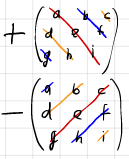
\includegraphics[width=.15\textwidth]{Dateien/00/14Sarrus.PNG}
\end{tabular}
\end{Satz}
\begin{Beispiel}
{Anwendung: Regel von Sarrus}
\begin{equation*}
    \det\Matrix{1&2&3\\4&5&0\\2&3&4}=1\cdot5\cdot4+2\cdot0\cdot2+4\cdot3\cdot3-4\cdot2\cdot4-1\cdot3\cdot0-2\cdot5\cdot3=20+36-32-30=-6
\end{equation*}
\end{Beispiel}
\begin{Satz}
{Rechenregeln}{Erlaubte Umformungen für Determinanten}
Beim Berechnen von Determinanten \underline{ändert sich nichts am Wert}, wenn wir
\begin{enumerate}
    \item Spalten vertauschen und dabei jeweils mit -1 multiplizieren:
    \blue{\begin{equation*}
        \det\Matrix{a&b&c\\d&e&f\\g&h&i}=-\det\Matrix{a&c&b\\d&f&e\\g&i&h}
    \end{equation*}}
    \item Vielfaches von Spalten zu anderen hinzuaddieren:
    \blue{\begin{equation*}
        \det\Matrix{a&b\\c&d}=\det\Matrix{a&b+2a\\c&d+2c}
    \end{equation*}}
    \item Die Matrix transponieren:
    \blue{\begin{equation*}
        \det A=\det\Matrix{a&b&c\\d&e&f\\g&h&i}=\det\Matrix{a&d&g\\b&e&h\\c&f&i}=\det A^T
    \end{equation*}}
\end{enumerate}
\blue{Aus der letzten Aussage ergibt sich, dass Zeilenumformungen genauso erlaubt sind wie Spaltenumformungen. Wir dürfen also quasi den Gauß-Algorithmus auf $A$ anwenden, nur dass wir Zeilen/Spalten nicht einfach vervielfachen dürfen und bei Vertauschungen aufpassen müssen.}
\end{Satz}
\begin{Satz}
{Rechenregel}{Determinanten mit Blockdreiecksmatrizen}
Die Determinante einer Blockdreiecksmatrix $E\in\Met(n+m,\mathbb{K})$, die sich aus den Matrizen $A\in\Met(n,\mathbb{K})$, $B\in\Met(n,m,\mathbb{K})$ und $D\in \Met(n,\mathbb{K})$ und der $m\times n$-Nullmatrix $\Vec{0}$ zusammensetzt, ist das Produkt der Determinanten von $A$ und $D$, d. h.
\begin{equation}
    \det\Matrix{A&B\\\Vec{0}&D}=\det A\cdot \det D.
\end{equation}
\end{Satz}
Aufgrund dieses Satzes reicht es auch, die Hauptdiagonalelemente miteinander zu multiplizieren, nachdem man erfolgreich den Quasi-Gaußalgorithmus\footnote{Wie gesagt, Achtung beim Vertauschen von Spalten/Zeilen und bei der Multiplikation mit Skalaren!} angewendet hat, d. h.
\begin{equation*}
    \det\Matrix{a_1& b &\cdots & c&d\\0&a_2&\cdots &e&f\\\vdots &  &\ddots & &\vdots\\0&0&\cdots &a_{n-1}&g\\0&0&\cdots &0&a_n}=\prod_{i=1}^na_i
\end{equation*}
\begin{Beispiel}
{Blockdreiecksmatrix (1/2)}
Wir können also ganz einfach die Determinante von folgender Monstermatrix berechnen:
\begin{equation*}
    \det\Matrix{1&2&3&4&5\\2&0&-2&4&6\\0&0&1&0&2\\0&0&2&1&0\\0&0&2&10&1}\overset{\footnote{Satz über Blockdreiecksmatrizen}}{=}\det\Matrix{1&2\\2&0}\det\Matrix{1&0&2\\2&1&0\\2&10&1}\overset{\footnote{Regel von Sarrus ergibt für die zweite Matrix $\det B=1+40+0-4-0-0=37$}}{=}(-4)37=-148.
\end{equation*}
\end{Beispiel}
\begin{Beispiel}
{Anwendung verschiedener Umformungen (2/2)}
Wir betrachten wieder die Matrix, die wir schon für die Regel von Sarrus kennengelernt hatten, und wollen auf verschiedene Weisen die Determinante bestimmen:\\
\begin{eqnarray*}
\det\Matrix{1&2&3\\4&5&0\\2&3&4}&\overset{\footnote{Transponieren}}{=}&\det\Matrix{1&4&2\\2&5&3\\3&0&4}\overset{\footnote{Erlaubte Umformung: $(II)- 2\cdot (I)$ und $(III)-3\cdot(I)$}}{=}\det\Matrix{1&4&2\\0&-3&-1\\0&-12&-2}\\
&\overset{\footnote{Satz zur Blockdreiecksmatrix}}{=}&\det(1)\det\Matrix{-3&-1\\-12&-2}\overset{\footnote{$\det (1)=1$, da es die $1\times 1$ Einheitsmatrix ist.\\Zudem nutzen wir die Linearität der Spalten, um die Faktoren $-3$ und $-1$ herauszuziehen}}{=}1(-3)(-1)\det\Matrix{1&1\\4&2}\\
&\overset{\footnote{Umformung: $(II)-4(I)$}}{=}&+3\Matrix{1&1\\0&-2}\overset{\footnote{Blockdreiecksmatrix}}{=}3\det(1)\det(-2)=-6
\end{eqnarray*}
Ein andere Möglichkeit wäre die Erzeugung der Stufenform:
\begin{eqnarray*}
\det\Matrix{1&2&3\\4&5&0\\2&3&4}&=&\det\Matrix{1&2&3\\0&-3&-12\\0&-1&-2}\overset{\footnote{Vertauschen zweier Zeilen, daher $(-1)$}}{=}-\det\Matrix{1&2&3\\0&-1&-2\\0&-3&-12}\\
&=&\det\Matrix{1&2&3\\0&-1&-2\\0&0&-6}=(-1)(-1)(-6)=-6.
\end{eqnarray*}
\end{Beispiel}

\subsubsection{Der Laplace'sche Entwicklungssatz}
Um den nächsten wichtigen Satz einzuführen, benötigen wir folgenden Begriff:
\begin{Def}
{Streichungsmatrix}
\begin{wrapfigure}{r}[0pt]{.35\textwidth}
 \vspace{-30pt}
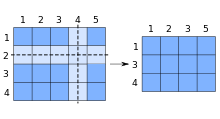
\includegraphics[width=.35\textwidth]{Dateien/01/01Submatrix_qtl1.svg.png}
 \vspace{-15pt}
\end{wrapfigure}
Für eine quadratische Matrix $A=(a_{kl})\in\Met(n,\mathbb{K})$ nennen wir $A_{ij}\in\Met(n-1,\mathbb{K})$ die ($i,j$)-te \red{Streichungsmatrix}\footnote{wobei $i,j\in\{1,...,n\}$. Dieser Begriff ist unter \href{https://de.wikipedia.org/wiki/Untermatrix}{Wikipedia} unter dem Namen 'Untermatrix' zu finden.}, die aus $A$ durch das Streichen der $i$-ten Zeile und $j$-ten Spalte entsteht.
\end{Def}
Durch den Laplace'schen Entwicklungssatz lässt sich die Berechnung der Determinante auf die Berechnung einiger 'kleinerer' Determinanten reduzieren.\\
Hierfür kann man eine Matrix $A$ nach der $i$-ten oder der $j$-ten Spalte \textit{entwickeln}:
\begin{Satz}{Satz}{Entwicklungssatz von Laplace}
Für die Determinante einer Matrix $A=(a_{kl})\in\Met(n,\mathbb{K})$ gilt
\begin{equation}
    \det A=\sum_{j=1}^n(-1)^{i+j}a_{ij}\det A_{ij}.
\end{equation}
\end{Satz}
Das sieht ziemlich wild aus, ist aber tatsächlich recht einfach:\\
Wir schnappen uns z.B. die erste Zeile und multiplizieren deren Einträge mit den Determinanten der Streichungsmatrizen und ggf. noch mit $(-1)$.
Wann ihr mit $(-1)$ multiplizieren müsst, könnt ihr euch nach folgendem Muster merken:
\begin{center}
    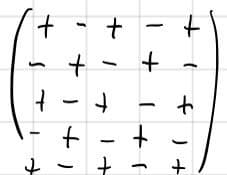
\includegraphics[width=.15\textwidth]{Dateien/01/01Laplacschema.jpg}
\end{center}
Es ist also immer alternierend.\\
\blue{\textbf{Hinweis}:\\
Es ist egal, nach welcher Zeile oder Spalte ihr entwickelt. Es lohnt sich häufig, gerade die Spalten/Zeilen zu wählen, die viele Nullen enthalten.}\\
Für das Beispiel, das wir auch im \textit{Determinanten}-Kapitel betrachtet hatten, sieht das dann so aus:
\begin{Beispiel}{Determinanten mit dem Entwicklungssatz berechnen}
Wir führen eine Entwicklung nach der ersten Zeile durch:
\begin{align*}
\det\Matrix{1&2&3\\4&5&0\\2&3&4}&=(-1)^{1+1}1\det\Matrix{5&0\\3&4}+(-1)^32\det\Matrix{4&0\\2&4}+3\det\Matrix{4&5\\2&3}\\
&=20-2\cdot16+3(12-10)=-12+6=-6.
\end{align*}
Alternativ können wir auch nach der dritten Spalte entwickeln:
\begin{align*}
\det\Matrix{1&2&3\\4&5&0\\2&3&4}&=(-1)^{1+3}3\det\Matrix{4&5\\2&3}+0+(-1)^{3+3}4\det\Matrix{1&2\\4&5}\\
&=3\cdot2+4(-3)=-6.
\end{align*}
\end{Beispiel}
Abschließend noch ein schönes Beispiel:
\begin{Beispiel}{Determinanten-Induktion}
\Zz{Für $n\in\mathbb{N}\setminus\{0\},\,a,b\in\mathbb{K}^n$ ist die Determinante einer Matrix $A$ der folgenden Gestalt durch
\begin{equation*}
    \det A=\det \Matrix{a_1&0&\cdots &\cdots&0&b_1\\
    0&\ddots&&&\iddots &0\\
    \vdots&&a_n&b_n&&\vdots\\
    \vdots&&b_n&a_n&&\vdots\\
    0&\iddots&&&\ddots &0\\
    b_1&0&\cdots &\cdots&0&a_1}=\prod_{k=1}^n(a_k^2-b_k^2)
\end{equation*}
gegeben.}
\Zb{Vollständige Induktion:\\
Induktionsanfang:\\
Für $n=1$ ist $\det A=\det\MatrixInline{a_1&b_1\\b_1&a_1}=a_1^2-b_1^2=\prod_{k=1}^n(a_k^2-b_k^2)$.\\
Es gelte die Induktionsvoraussetzung (siehe Aussage) für $n\geq 1$.\\
Induktionsschritt:\\
So folgt die Aussage für $n+1$, denn:
\begin{eqnarray*}
    \det A&=&\MatrixAbs{a_1&0&\cdots &\cdots&0&b_1\\
    0&\ddots&&&\iddots &0\\
    \vdots&&a_{n+1}&b_{n+1}&&\vdots\\
    \vdots&&b_{n+1}&a_{n+1}&&\vdots\\
    0&\iddots&&&\ddots &0\\
    b_1&0&\cdots &\cdots&0&a_1}\\
    &\overset{\footnote{Laplace-Entwicklung nach der $n+1$-ten Zeile}}{=}&a_{n+1}\MatrixAbs{a_1&0&\cdots &0&b_1\\
    0&\ddots&&\iddots &0\\
    \vdots&&a_{n+1}&&\vdots\\
    0&\iddots&&\ddots &0\\
    b_1&0&\cdots &0&a_1}-b_{n+1}\MatrixAbs{a_1&0&\cdots &0&b_1\\
    0&\ddots&&\iddots &0\\
    \vdots&&b_{n+1}&&\vdots\\
    0&\iddots&&\ddots &0\\
    b_1&0&\cdots &0&a_1}
\end{eqnarray*}
\begin{eqnarray*}
    &\overset{\footnote{Erneute Entwicklung nach der $n+1$-ten Zeile}}{=}&a_{n+1}^2\MatrixAbs{a_1&0&\cdots &\cdots&0&b_1\\
    0&\ddots&&&\iddots &0\\
    \vdots&&a_{n}&b_{n}&&\vdots\\
    \vdots&&b_{n}&a_{n}&&\vdots\\
    0&\iddots&&&\ddots &0\\
    b_1&0&\cdots &\cdots&0&a_1}-b_{n+1}^2\MatrixAbs{a_1&0&\cdots &\cdots&0&b_1\\
    0&\ddots&&&\iddots &0\\
    \vdots&&a_{n}&b_{n}&&\vdots\\
    \vdots&&b_{n}&a_{n}&&\vdots\\
    0&\iddots&&&\ddots &0\\
    b_1&0&\cdots &\cdots&0&a_1}\\
    &\overset{\footnote{Nutze die Induktionsvoraussetzung}}{=}&a_{n+1}^2\prod_{k=1}^n(a_k^2-b_k^2)-b_{n+1}^2\prod_{k=1}^n(a_k^2-b_k^2)\\
    &=&(a_{n+1}^2-b_{n+1}^2)\prod_{k=1}^n(a_k^2-b_k^2)\\
    &=&\prod_{k=1}^{n+1}(a_k^2-b_k^2)
\end{eqnarray*}}
\end{Beispiel}

\begin{Satz}
{Rechenregeln}{Zusammenfassung weiterer wichtiger Eigenschaften}
Wie wir gesehen hatten, gilt für $A, B, \mathds{1}_n\in\mathbb{N}$:
\begin{itemize}
    \item $\det(\mathds{1}_n)=1$
    \item $\det(A)=\det(A^T)$
    \item $\det(AB)=\det(A)\det(B)$
    \item $\det(A^{-1})=\det(A)^{-1}$ falls $\det (A)\neq0$.
\end{itemize}
\end{Satz}
\blue{\textbf{Tipp}:\\
Das Video \textbf{The Determinant} von 3Blue1Brown auf Youtube (unter \href{https://youtu.be/Ip3X9LOh2dk}{diesem Link} zu finden) erklärt sehr anschaulich die geometrische Bedeutung der Determinante als Maß für das Volumen der geometrischen Figur, auf die die Einheitsvektoren abgebildet werden.\\
Unserer Meinung nach bietet der Kanal generell sehr anschauliche Videos zu mathematischen Themen.}

\subsection{Zeit, umzukehren}
Wir betrachten nun einige Werkzeuge zum Invertieren von Matrizen. Dazu kurz nochmal ein Rückblick:
\begin{Wiederholung}{Lemma zur Bijektivität und Umkehrabbildung}\label{satz:BijektivitatUmkehrabbildung}
Eine Abbildung $f:A\rightarrow B$ ist \underline{genau dann bijektiv}, falls es eine Abbildung $g:B\to A$ gibt (diese nennen wir dann \red{Umkehrabbildung}), die die folgenden Relationen erfüllt:
\begin{equation}
    g\circ f=\text{Id}_A\,\wedge\, f\circ g=\text{Id}_B.\label{eq:Umkehrabbildung}
\end{equation}
\end{Wiederholung}
Wie wir schon festgestellt hatten, ist eine Matrix $A\in\Met(n,\mathbb{K})$ genau dann \red{invertierbar}, wenn $\det A\neq 0$.\\
Was bedeutet aber \textit{invertierbar}?
\begin{Wiederholung}{Inverse Matrix}
Ist $A$ invertierbar, so existiert eine \red{zu $A$ inverse Matrix $A^{-1}$}, sodass gilt:
\begin{equation}
    A\cdot A^{-1}=\mathds{1}_n\quad\tx{und}\quad A^{-1}\cdot A=\mathds{1}_n.
\end{equation}
\end{Wiederholung}
Falls $A$ die darstellende Matrix eines Endomorphismus ist, so ist dieser dann bijektiv und wir nennen ihn \red{Automorphismus}. Seht ihr die Parallelen zum Lemma zur Umkehrabbildung?\
\begin{Beispiel}{Inverse Matrix}
Sei $A=\Matrix{2&2\\3&4}$.\\
\Zz{Die Matrix $A^{-1}=\Matrix{2&-1\\-\frac{3}{2}&1}$ ist die zu $A$ inverse Matrix.}
\Zb{Es gilt 
\begin{equation*}
    A\cdot A^{-1}=\Matrix{2&2\\3&4}\Matrix{2&-1\\-\frac{3}{2}&1}=\Matrix{4-3&-2+2\\6-6&-3+4}=\Matrix{1&0\\0&1}=\mathds{1}_2
\end{equation*}
und analog andersherum.}
\end{Beispiel}

\begin{Wiederholung}{Inverse einer Determinante}
Für alle Gruppenhomomorphismen gilt $\phi(a^{-1})=\phi(a)^{-1}$. Somit gilt für alle\\
$A\in\GL(n,\mathbb{K})$:
\begin{equation}
    \det(A^{-1})=\det(A)^{-1}.
\end{equation}
Dies ist wohldefiniert, da $A\in\GL(n,\mathbb{K})$ per Definition bijektiv ist und somit eine Umkehrabbildung $A^{-1}$ besitzt und die Determinante nicht verschwindet.
\end{Wiederholung}
\begin{Wiederholung}
{Anwendung der Inversen Determinante}
Sei $A=\Matrix{2&2\\3&4}$. Die inverse Matrix ist (wie eben gesehen) $A^{-1}=\Matrix{2&-1\\-\frac{3}{2}&1}$.\\
Somit gilt:
\begin{align*}
    \det(A^{-1})&=2-(-1)(-3/2)=2-\frac{3}{2}=\frac{1}{2}\\
    \det(A)^{-1}&=(2\cdot 4-3\cdot 2)^{-1}=2^{-1}=\frac{1}{2}.
\end{align*}
\end{Wiederholung}
\begin{Def}
{Spezielle lineare Gruppe}
Wir bezeichnen die Untergruppe aller Automorphismen mit $\det A=1$ als \red{spezielle lineare Gruppe} und schreiben
\begin{equation}
    \SL=\Menge{A\in \GL(n,\mathbb{K})}{\det A=1}\subset \GL(n,\mathbb{K}).
\end{equation}
\end{Def}


\subsubsection{Invertieren mit dem Gauß-Verfahren}
Wie finden wir aber nun die inverse Matrix zu einer gegebenen Matrix $A$?
\begin{Satz}
{Rechenregel}{Invertieren einer Matrix mit Gauß}
Die erste Idee ist, dass wir ein Gleichungssystem umwandeln, indem wir mit $A^{-1}$ multiplizieren, d. h.
\begin{equation*}
    A\xvec=\Hat{\Vec{e}}_i\to \xvec=A^{-1}\Hat{\Vec{e}}_i.
\end{equation*}
Eine solche Überführung können wir durch den Gaußschen Algorithmus erreichen.\\
Um das für alle Spalten von $A^{-1}$ gleichzeitig zu machen, lösen wir also $(A\furdas\mathds{1}_n)\to(\mathds{1}_n\furdas A^{-1})$.
\end{Satz}
Das hört sich vielleicht komplizierter an, als es ist, daher hier ein Beispiel.
\begin{Beispiel}
{Invertieren einer Matrix mit Gauß}
Wir wollen die Matrix $A\in \GL(3,\mathbb{R}),\,A=\MatrixInline{1&2&3\\2&1&-1\\0&0&2}$ invertieren:
\begin{align*}
    (A\furdas\mathds{1}_3)&=\MatrixInvertieren{1&2&3\\2&1&-1\\0&0&2}{1&0&0\\0&1&0\\0&0&1}\overset{\tx{II}-2\tx{I},\, \tx{III }/2}{\longrightarrow}\MatrixInvertieren{1&2&3\\0&-3&-7\\0&0&1}{1&0&0\\-2&1&0\\0&0&1/2}\\
    \overset{\tx{I}-3\tx{III},\,\tx{II}+7\tx{III}}&{\longrightarrow}\MatrixInvertieren{1&2&0\\0&-3&0\\0&0&1}{1&0&-3/2\\-2&1&7/2\\0&0&1/2}\overset{\tx{II}/(-3)}{\longrightarrow}\MatrixInvertieren{1&2&0\\0&1&0\\0&0&1}{1&0&-3/2\\2/3&-1/3&-7/6\\0&0&1/2}\\
    \overset{\tx{I}-2\tx{II}}&{\longrightarrow}\MatrixInvertieren{1&0&0\\0&1&0\\0&0&1}{-1/3&2/3&5/6\\2/3&-1/3&-7/6\\0&0&1/2}=(\mathds{1}_3\furdas A^{-1}).
\end{align*}
Somit ist $A^{-1}=\frac{1}{6}\MatrixInline{-2&4&5\\4&-2&-7\\0&0&3}$ die zu $A$ inverse Matrix.\\
Wie können wir das testen?
\begin{itemize}
    \item \textbf{Überprüfe die Determinanten}:\\
    $\det(A^{-1})\overset{!}{=}(\det A)^{-1}$. Es ist
    \begin{eqnarray*}
        \det(A^{-1})&\overset{\footnote{Regel von Sarrus, Linearität}}{=}&\BracedIn{\frac{1}{6}}^3\BracedIn{(-2)(-2)3-4\cdot4\cdot3}=\frac{1}{36}\BracedIn{2-8}=-\frac{6}{36}=-\frac{1}{6}.\\
        \det A&=&1\cdot 1\cdot 2-2\cdot 2\cdot 2=2-8=-6\implies (\det A)^{-1}=-\frac{1}{6}.
    \end{eqnarray*}
    Leider ist dieses Kriterium nur notwendig, aber nicht hinreichend. Es kann aber als schneller Test dienen.
    \item \textbf{Stumpf rechnen}:\\
    Wir berechnen einfach
    \begin{equation*}
        A\cdot A^{-1}=\frac{1}{6}\Matrix{-2&4&5\\4&-2&-7\\0&0&3}\Matrix{1&2&3\\2&1&-1\\0&0&2}\overset{\footnote{Wir tun an dieser Stelle einfach mal so, als hätten wir das wirklich gerechnet ;)}}{=}\Matrix{1&0&0\\0&1&0\\0&0&1}.
    \end{equation*}
    Dieses Kriterium ist dann sowohl notwendig als auch hinreichend.
\end{itemize}
\end{Beispiel}

\subsubsection{Invertieren mit der Adjunkten}
Es gibt eine weitere, unintuitivere Möglichkeit, Matrizen zu invertieren. Hierfür benötigen wir den Begriff der adjunkten Matrix:
\begin{Def}
{Adjunkte Matrix}
Für die Matrix $A=(a_{ij})_{ij}\in\Met(n,\mathbb{K})$ definieren wir die \red{adjunkte Matrix} $\Tilde{A}=(\Tilde{a}_{ij})_{ij}$, die die folgenden Einträge hat:
\begin{equation*}
    \Tilde{a}_{ij}=(-1)^{i+j}\det A_{ji}=\det(\Vec{a}_1\ldots\Vec{a}_{i-1}\Vec{e}_j\Vec{a}_{i+1}\ldots a_n),
\end{equation*}
wobei $A_{ji}$ die $ji$-te Streichungsmatrix ist.
\end{Def}
Das sieht auf den ersten Blick erst mal ungewohnt aus, also betrachten wir es genauer:
\begin{Beispiel}
{Adjunkte einer $2\times 2$-Matrix (1/2)}
Sei $A=\MatrixInline{a&b\\c&d}$, so finden wir
\begin{equation*}
    \Tilde{a}_{11}=(-1)^2\det d,\quad \Tilde{a}_{12}=(-1)^3\det b,\quad \Tilde{a}_{21}=(-1)^3\det c,\quad \Tilde{a}_{22}=(-1)^4\det a. 
\end{equation*}
Somit ist $\Tilde{A}=\MatrixInline{d&-b\\-c&a}$.
\end{Beispiel}
\begin{Beispiel}
{Adjunkte einer $3\times 3$-Matrix (2/2)}
Sei $A=\MatrixInline{a&b&c\\d&e&f\\g&h&i}$, so finden wir
\begin{equation*}
    \Tilde{a}_{11}=(-1)^2\det \Matrix{e&f\\h&i},\quad \Tilde{a}_{12}\overset{\footnote{Streichungsmatrix 2. Zeile, 1. Spalte}}{=}(-1)^3\det \Matrix{b&c\\h&i},\quad \Tilde{a}_{13}=(-1)^4\det\Matrix{b&c\\e&f}
\end{equation*}
und so weiter...
\end{Beispiel}
\begin{Satz}
{Satz}{Zur adjunkten Matrix}
Für die adjunkte Matrix $\Tilde{A}$ zu $A\in \Met(n,\mathbb{K})$ gilt:
\begin{equation}
    A\cdot \Tilde{A}=\det A\mathds{1}_n\quad\tx{und}\quad \Tilde{A}\cdot A=\det A\mathds{1}_n.
\end{equation}
\end{Satz}
Wir sehen also, dass die Adjunkte quasi die Struktur der inversen Matrix hat, jedoch um einen Faktor $\det A$ daneben liegt.
\begin{Satz}
{Rechenregel}{Cramersche Regel zur Bestimmung der inversen Matrix}
Mithilfe der Adjunkten können wir aufgrund des vorhergehen Satzes also leicht die inverse Matrix einer invertierbaren Matrix $A\in\GL(n,\mathbb{K})$ bestimmen, denn es gilt
\begin{equation}
    \boxed{A^{-1}=\frac{1}{\det A}\Tilde{A}}.
\end{equation}
\end{Satz}
Der folgende Satz ist recht wichtig, es lohnt sich, ihn auswendig zu lernen:
\begin{Satz}
{Merksatz}{Inverse einer $2\times2$-Matrix}
Sehr häufig braucht man das Inverse einer $2\times2$-Matrix $A=\MatrixInline{a&b\\c&d}$.\\
Mithilfe der Adjunkten sehen wir:
\begin{equation}
    \label{eq:01InverseZweiKreuzZwei}A^{-1}=\frac{1}{\det A}\Tilde{A}=\frac{1}{ad-bc}\Matrix{d&-b\\-c&a}.
\end{equation}
\end{Satz}





\subsection{Exkurs: Volumen eines Parallelotops}\label{ssec:14AnhangParallelotop}
Hier wie versprochen noch ein schöner 'Appetithappen' zur Anwendung der Determinante

\begin{Beispiel}{Volumen eines Parallelotops}
Ein Parallelotop in einem $n$-dimensionalen Raum wird von $n$ Vektoren aufgespannt. Im Zweidimensionalen nennt man es
Parallelogramm, im Dreidimensionalen Parallelepiped.

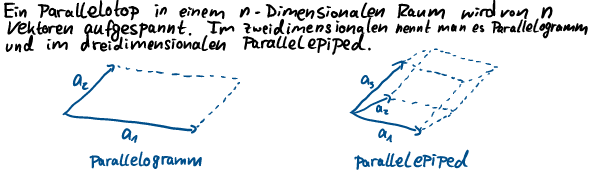
\includegraphics[width=0.8\textwidth]{Dateien/00/14Parallelotop1.png}

Die mathematische Definition lautet für $n$ Dimensionen:
\begin{equation}
    P(a_1, \ldots, a_n) = \{ x = \sum_{i=1}^n \lambda_i a_i | \lambda_1, \ldots, \lambda_n \in [0,1] \}
\end{equation}
Wir definieren für das Volumen:
\begin{equation}
    V(P(a_1, \ldots, a_n)) \eqqcolon V(a_1, \ldots, a_n) \eqqcolon V\overbrace{(a_1 \ldots a_n)}^{\substack{\text{Dies
    kann man als eine}\\ n\times n\text{ Matrix auffassen, mit den}\\\text{Vektoren }a_i\text{als Spalten}}}
\end{equation}
Es gibt hier noch eine kleine Feinheit: Sind die Vektoren $a_1, \ldots, a_n$ rechtshändig angeordnet, nennt man das
Parallelotop \red{positiv orientiert}, das Volumen ist somit positiv. Sind die Vektoren umgekehrt linkshändig
angeordnet, nennt man das Volumen \red{negativ orientiert}, das Volumen ist also negativ (ja, in der Mathematik darf man
das). Der Orientierungsbegriff wird euch noch oft wieder begegnen, hier hat er seinen Ursprung. Also unbedingt im
Hinterkopf behalten!

Für das Volumen eines Parallelotops stellen wir die folgenden Regeln fest:
\begin{enumerate}
    \item $V(a_1\ldots \mu a_i + \lambda b_i \ldots a_n) = \mu V(a_1 \ldots a_i \ldots a_n) + \lambda V(a_1 \ldots b_i
        \ldots a_n)$ mit $\mu, \lambda \in \mathds{R}$
    \item $a_i, a_j$ linear abhängig $\Rightarrow V(a_1 \ldots a_i \ldots a_j \ldots a_n) = 0$
    \item $V(e_1, \ldots, e_n) = 1$
\end{enumerate}
Die Begründung zeigen wir hier für $n=2$, sie sollte aber recht intuitiv auf beliebige Dimensionen erweiterbar sein.

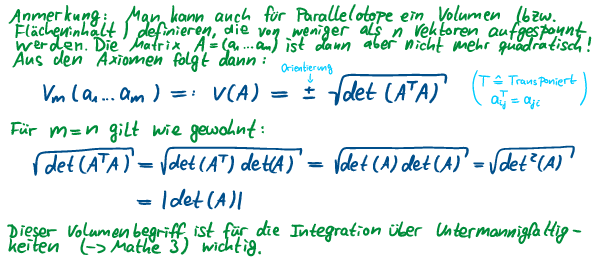
\includegraphics[width=0.8\textwidth]{Dateien/00/14Parallelotop2.png}

Ein strikter Beweis ist im Königsberger, Analysis 2 zu finden. Dort wird allerdings die Orientierung unterbunden, indem
der Betrag der Determinante genommen wird.\\
Damit sind wir auch schon beim Clou der ganzen Geschichte: Die Axiome
beider Methoden sind exakt gleich! Es gilt also:
\begin{equation}
    V(a_1\ldots a_n) = \det(a_1\ldots a_n)
\end{equation}

Anmerkung: Man kann auch für Parallelotope ein Volumen (bzw. Flächeninhalt) definieren, die von weniger als $n$ Vektoren
aufgespannt werden. Die Matrix $A=(a_1\ldots a_n)$ ist dann aber nicht mehr quadratisch! Aus den Axiomen folgt dann:
\begin{equation}
    V_m(a_1\ldots a_m) \eqqcolon V(A) = \overbrace{\pm}^{\text{Orientierung}} \sqrt{\det(A^TA)}
\end{equation}
Für $m=n$ gilt wie gewohnt:
\begin{gather}
    \sqrt{\det(A^TA)} = \sqrt{\det(A^T)\det(A)} = \sqrt{\det(A)\det(A)} = \sqrt{{\det}^2(A)} = |\det(A)| \\
    \text{mit } (a_{ij})^T = a_{ji} \text{ (transponiert)}\notag
\end{gather}
Dieser Volumenbegriff ist für die Integration über Untermannigfaltigkeiten ($\to$ Mathe 3) wichtig.
\end{Beispiel}


\subsection{Exkurs: Anwendung von Gruppen - Symmetrietransformationen}\label{ssec:ExkursSymTrafos}
Das Folgende ist nicht Teil der Mathevorlesung und vor allem für Interessierte gedacht. Ein paar Sachen werden euch dabei vielleicht in den Vorlesungen zur Quantenmechanik wiederbegegnen... \\
\begin{Beispiel}{Translationsgruppe (1/2)}
Schauen wir uns zunächst einmal die Translationsgruppe $T$ für eine Funktion \linebreak $f:\mathbb{R} \rightarrow \mathbb{R}$ an. Diese Gruppe besteht aus Elementen $t_{a}$, $a \in \mathbb{R}$, die wie folgt auf die Funktion wirken:
\begin{equation*}
    t_{a}f(x)=f(x+a).    
\end{equation*}
Sie verschieben also das Argument der Funktion um $a$. Es ist schnell zu erkennen, dass es ein inverses Element $t_{-a}$ und ein neutrales Element $t_{0}$ gibt, wenn wir die (assoziative) Verknüpfung wie folgt wählen:
\begin{equation*}
    t_{a}\cdot t_{b} = t_{a+b}.
\end{equation*}
Können wir nun eine spezielle Darstellung der Gruppenelemente finden? Aber klar! Dazu schauen wir uns eine infinitesimale Verschiebung $t_{da}$ an und erinnern an die Definition des Differenzenquotienten (denn wir hier mal auf Physikerart hinschreiben):
\begin{align*}
    \frac{df}{dx}=&\frac{f(x+da)-f(x)}{da} \\
    &\Rightarrow t_{da}f(x) = f(x+da) = f(x)+da \cdot \frac{df}{dx} = \big( 1 + da\frac{d}{dx} \big) f(x)
\end{align*}
Jetzt nutzen wir die Definition der Verknüpfung aus und erhalten für beliebige Transformationen:
\begin{align*}
    t_{a} = t_{\frac{a}{2}}\cdot t_{\frac{a}{2}} = ... &= \lim_{N \rightarrow \infty} \big( t_{\frac{a}{N}} \big)^{N} = \lim_{N \rightarrow \infty} \big( 1 + \frac{a}{N} \frac{d}{dx} \big)^{N} \\ 
    &= \exp{(a\frac{d}{dx})}
\end{align*}
Dabei haben wir benutzt, dass $a/N$ für große $N$ sehr klein und damit zu $da$ wird. Außerdem haben wir die Grenzwertdarstellung der Exponentialfunktion verwendet, die noch aus dem ersten Semester bekannt sein sollte. \\
Das interessante Ergebnis unserer kleinen Rechnung ist also:
\begin{equation*}
    t_{a}f(x)=\exp{(a\frac{d}{dx})}f(x) = f(x+a)
\end{equation*}
womit wir eine explizite Darstellung gefunden haben. Genau genommen nennt man das Argument der Exponentialfunktion ohne den Parameter $a$, also $d/dx$, die (Operator-)Darstellung der Translationsgruppe.
\end{Beispiel}
\begin{Beispiel}{Rotationsgruppe (2/2)}
Diese Art von Rechnung ist zum Beispiel in der Quantenmechanik sehr nützlich und kann auch auf Rotationen angewendet werden.\\
Die Rotationsgruppe\footnote{Wenn ihr Normen einführt, werdet ihr Lernen, dass diese Matrizen die Länge eines Vektors unverändert lassen und wegen $\det(R)=1$ keine Spiegelungen enthalten.} ist gegeben durch die spezielle orthogonale Gruppe $\text{SO}(N)$, wobei 
\begin{equation*}
    \text{SO}(N) := \Menge{R \in \Met(n,\mathbb{R})}{RR^{T}=R^{T}R=\mathds{1} \land \det(R) = 1}.
\end{equation*}
Der Einfachheit halber wollen wir hier nur Rotationen um die z-Achse in drei Dimensionen betrachten, die durch die wohlbekannte Matrix
\begin{equation*}
    R_{\theta} = \Matrix{\cos(\theta) & -\sin(\theta) & 0 \\ \sin(\theta) & \cos(\theta) & 0 \\ 0 & 0 & 1}
\end{equation*}
gegeben sind.\\
Eine Rotation $r_{\theta}$ einer Funktion $f:\mathbb{R}^{3} \rightarrow \mathbb{R}$ ist dann gegeben durch:
\begin{equation*}
    r_{\theta}f(v) = f(R_{\theta} v).
\end{equation*}
Diese Transformationen $r_{\theta}$ bilden aus denselben Gründen wie bei den Translationen eine Gruppe. \\
Können wir auch hier wieder eine explizite Darstellung finden? Aber natürlich! Dazu schauen wir uns abermals ein infinitesimale Transformation an und beachten dafür die Kleinwinkelnäherung $\sin(d\theta)=d\theta$ und $\cos(d\theta)=1$:
\begin{equation*}
    R_{d\theta}=\Matrix{1 & -d\theta & 0 \\ d\theta & 1 & 0 \\ 0 & 0 & 1}.
\end{equation*}
Daraus folgt:
\begin{equation*}
    r_{d\theta}f(v) = f(R_{d\theta}v) = f(x-yd\theta, y+xd\theta, z)
\end{equation*}
Jetzt packen wir den Zauberstab aus und spielen ein wenig mit den Differentialen herum, aber versprochen, es funktioniert! Im Differenzenquotienten packen wir erstmal einfach ein konstantes $y$ und $x$ hinzu, was uns ja keiner verbietet ($yd\theta$ ist ja immernoch sehr klein):
\begin{align*}
    \frac{df}{dx}&=\frac{f(x+(-yd\theta),y,z)-f(x,y,z)}{-yd\theta} \Leftrightarrow f(x-yd\theta,y,z)=(1-yd\theta\frac{d}{dx})f(x,y,z) \\
    \frac{df}{dy}&=\frac{f(x,y+xd\theta,z)-f(x,y,z)}{xd\theta} \Leftrightarrow f(x,y+xd\theta,z) = (1+xd\theta\frac{d}{dx})f(x,y,z)
\end{align*}
Daraus folgt, wenn wir annehmen, dass $d\theta^{2}$ sehr klein und somit vernachlässigbar ist:
\begin{align*}
    f(x-yd\theta,&y+xd\theta,z) = (1-yd\theta\frac{d}{dx})f(x,y+xd\theta,z)\\ &= (1-yd\theta\frac{d}{dx})(1+xd\theta\frac{d}{dx})f(x,y,z) = (1+xd\theta\frac{d}{dx}-yd\theta\frac{d}{dx})f(x,y,z).
\end{align*}
Wir haben also für die infinitesimale Rotation gefunden:
\begin{equation*}
    r_{d\theta}f(v)=(1+d\theta(x\frac{d}{dx}-y\frac{d}{dx}))f(v).
\end{equation*}
Das sieht doch schon mal richtig gut aus! Tatsächlich können wir hier den gleichen Trick wie bei der Translationsgruppe benutzen, um diese Vorschrift zu verallgemeinern:
\begin{align*}
    r_{\theta}f(v) = (r_{\frac{\theta}{2}})^{2}f(v)&=...=\lim_{N\rightarrow\infty}(r_{\frac{\theta}{N}})^{N}f(v)=\lim_{N\rightarrow\infty}(1+\frac{\theta}{N}(x\frac{d}{dx}-y\frac{d}{dy}))^{N}f(v)\\ &=\exp{(\theta(x\frac{d}{dy}-y\frac{d}{dx})}f(v) =: \exp{(\theta L)}f(v)
\end{align*}
Wir haben also tatsächlich eine (Operator-)Darstellung der Rotationsgruppe gefunden! Sie lautet:
\begin{equation*}
    L:=x\frac{d}{dy}-y\frac{d}{dx}.
\end{equation*}
\end{Beispiel}
Wir hoffen, dass diese doch etwas verschwurbelte Rechnung einigermaßen verständlich war. Sollte sie zu Verwirrung geführt haben, vergesst einfach die letzten beiden Seiten und konzentriert euch auf den wesentlichen Stoff! Vielleicht hat es ja trotzdem bei dem/der ein oder anderen, der/die auch schon Quantenmechanik (Physik 3) gehört und $L$ als den berühmten Drehimpulsoperator (oder besser gesagt seine z-Komponente) erkannt hat, zu einem Aha-Erlebnis geführt. Es sind unserer Meinung nach einfach zwei sehr schöne Beispiele für die Verwendung von Gruppen.

\Tipps{1}{
\begin{enumerate}
    \item Die Formulierung ist vielleicht etwas ungewohnt, aber fasst einfach die Polynome als Vektor auf und sucht euch zunächst ein Beispiel.\\
    Auf was wird z. B. das Polynom $P(x)=5+7x-3x^3=\MatrixInline{5\\7\\0\\-3}$ durch die Ableitung abgebildet?\\
    Dann müsst ihr euch überlegen, wie ihr diese lineare Abbildung mithilfe einer Matrix aufschreiben könnt.\\
    Alternativ könnt ihr auch ganz klassisch schauen, was die Ableitung mit den Basisvektoren der Basis $(1,x,x^2,x^3)$ macht, und wie ihr das Ergebnis durch diese wieder darstellen könnt. Spaltenweise aufgeschrieben ergibt das dann eure Matrix.\\
    Spur und Determinante sollten ein Kinderspiel sein.
    \item Auch bei dieser Aufgabe handelt es sich um relativ kurze Rechnungen. Bei a.) erinnert euch einfach daran, wie Linearität definiert ist. Auch bei b.) schaut euch an, was für Matrizen gelten muss, die im Kern von $\varphi$ liegen und welche Bedingungen daraus für die Matrixelemente folgen. In c.) müsst ihr das Bild auf Symmetrie untersuchen und euch überlegen, wie man beliebige symmetrische Matrizen so zerlegen kann, dass sie ein Bild von $\varphi$ sind. Für d.) schaut euch nochmal die Körperaxiome an.
    \item Determinanten zu berechnen ist eines der wichtigsten Werkzeuge dieses Semesters, also setzt euch in Ruhe daran und geht alle Sätze durch, die ihr dafür nutzen könntet - Eventuell ist es sogar sinnvoll, die Determinanten mit verschiedenen Wegen zu berechnen.\\
    Nützlich sind natürlich quasi-Gauß'sche Umformungen, der Satz über Blockdreiecksmatrizen, die Cramer'sche Regel, die Regel von Sarrus und der Laplace'sche Entwicklungssatz die gängigen Mittel.
    \item  
    \begin{enumerate}
        \item Hier hilft es, die Linearität der Determinante auszunutzen - welche Spalte bietet sich dafür an? Denkt dann an den Gauß-Algorithmus.\\
        Ihr solltet bei einem Ausdruck der Form
        \begin{equation*}
            \det A= \prod_{i=1}^n a_i+\sum_{k=1}^nb_k\prod_{j\neq k}^n c_j
        \end{equation*}
        kommen.
        \item Wir sehen leider nicht, wie man das mit Induktion macht, wir haben das mithilfe eines direkten Beweises und Aufgabe 3a) gemacht. Auch hier gilt wieder: Linearität ausnutzen!\\
        Weiterer Tipp (der in ähnlicher Form vielleicht nützlich ist):
        \begin{equation*}
            \det\Matrix{a_1&a_2&a_3\\a_1&a_2&a_3\\a_1&a_2&a_3}=\prod_{i=1}^3a_i\det\Matrix{1&1&1\\1&1&1\\1&1&1}
        \end{equation*}
    \end{enumerate}
\end{enumerate}
}


